%methods chapter
% Enough for an expert to reproduce without needing extensive references
% all data should be in thesis so they can be checked (appendix maybe and supplements)
% Methods commonly used throughout maybe leaving chapter specific methods to that chapter
\graphicspath{{chapters/2.Methods/figures}}

\chapter{Methods}

Materials and methods section

\begin{itemize}
    \item Sequencing - general sequencing background sanger -> 2nd gen
    \item Genomics/transcriptomics - how this is specifically applied via HiSeq
    \item Phylogenetics - general, alignment, masking, model selection, tree reconstructions 
    \item Dendrogenous - UML of database, flowchart of program, comparison of parallelisation, profiling of tools process-level parallelism vs built in parallellism
\end{itemize}

univariate mathematical distributions reference\citep{Leemis2008}




\section{Microbiology}


\subsection{Cultures}

During this project 3 \textit{Paramecium bursaria} cultures have been used at various stages from 
the UK Culture Collection of Algae and Protozoa (CCAP) and the Japanese National BioResource Project (NBRP).
Specifically:
\begin{itemize}
    \item CCAP 1660/12: European \textit{Paramecium bursaria} SW1 with \textit{Micractinium reisseri} SW1-ZK \citep{Hoshina2010}
    \item CCAP 1660/13: European \textit{Paramecium bursaria} with \textit{Coccomyxa} CCAP 216/24 \footnote{This is a mixed culture 
            containing both CCAP 1660/12 strain with \textit{Micractinium} and the \textit{Coccomyxa} bearing strain, 
        the \textit{Coccomyxa} endosymbiont has been further isolated in CCAP under the description CCAP 216/24 (pers. comm. Undine Achilles-Day CCAP)}
    \item NBRP Yad1g1N: Japanese \textit{Paramecium bursaria} Yad1w with \textit{Chlorella variabilis} 1N \footnote{
        Yad1g1N host is mating type 1 and was created by mixing of isolated and 
        cultured endosymbiont (\textit{Chlorella variabilis} Clone 1 (known as 1N strain)
        }
\end{itemize}

Both CCAP cultures (1660/12 and 1660/13) were isolated from the same pond in Cambridge, UK (pers. comm. Undine Achilles-Day CCAP)
CCAP 1660/12 was the principal culture and all genomic, transcriptomic and metabolomics analyses were conducted using these cultures. 
Theoretically, these 3 cultures provide us with \textit{Paramecium bursaria} strains harbouring members of each of the 3 species of 
green algal endosymbiont (see \ref{chap1} for more details).

\subsection{Media and Culture conditions}
All \textit{P. bursaria} and green algae cultures are maintained in 
New Cereal Leaf-Prescott Liquid (NCL) media 
(4.3g/l \(CaCl_{2}.2H$_{2}O\), 1.6g/l KCl, 5.1g/l \(K_{2}HPO_{4}\), 2.8g/l \(MgSO_{4}.7H_{2}O\), 
1g/l wheat bran, gravity filtered via GF/C paper and autoclaved) and stored in 
a 12:12 light:dark cycle incubator at 15\celsius. [\url{http://www.ccap.ac.uk/media/documents/NCL.pdf}].  
%2x21 watt 865 daylight tubes at 2000 lumen each
Cultures were sub-cultured every 2 weeks with fresh NCL media and were inspected using light microscopy to monitor health.  

No bacteria was provided in cultures using for transcriptomics or genomics but otherwise the medium was bacterised with
\textit{Klebsiella pneumoniae} SMC (strain donated by the Meyer Lab, Ecole Normale Supérieure, Paris) the day before use. 

\section{Omics}
``-omic'' technologies are those aimed at globally characterising a class of biomolecules 
within a specific biological sample (charactising the ``-ome''). The most prevalent and developed 
are genomics, transcriptomics, metabolomics and proteomics. 
Genomics aims to detect and analyse DNA, seeking to describe and discover genes and non-coding DNA
features. Similarly, transcriptomics is orientated around the characterisation
of mRNA in a sample and thus to investigate mRNA transcription, usually assessing
gene expression in response to a given condition or feature. 
Metabolomics, on the other hand, seeks to identify and quantify small biomolecules that make up the terminal and
intermediate products of cellular metabolism e.g. carbohydrates, alcohols, and animo acids.
Proteomics, on the other hand, is orientated towards the characterisation  
of proteins present in a sample. 
Furthermore, there are a plethora of different approaches which seek to characterise
different subsets of these biomolecules e.g. epigenomics (epigenetic modification to DNA such as methylation
and histone binding), gylcomics (characterisation of saccharides) and microbiomics (community genomics of organisms associated with a metazoan organism e.g. microbes present in the human digestive tract).
``Meta-\ldots-omics'' is the application of specific ``omic'' method to a biological sample 
containing multiple organisms. For example, ``metagenomics'' has been used to investigate
the cellular community composition of marine micro-eukaryotes \citep{}<++> (BIOMARKS PAPER WHEN PUBLISHED) %BIOMARKS PAPER WHEN PUBLISHED

The major utility of ``omic'' technologies is to globally identify and quantify key cellular components
in a largely non-biased manner (although many biases exist across the different platforms
relative to targeted approach focussing on a specific cellular component
e.g. abundance of a certain transcript using RT-PCR they are unbiased). 
Furthermore, while pre-existing databases and literature will aid analysis of omic datasets, 
they largely don't require as much \texit{a priori} knowledge of a specific organism or environment as a targeted approach.
Therefore, it is possible to investigate novel non-model organisms and systems.

However, care must be taken with ``omics'' approaches as they can easily become purely descriptive,
not provide explanatory or mechanistic insight, not generate testable hypotheses or produce
models without biological relevance \citep{Fang2011}. This is generally true
of so-called ``holistic'' or systems approaches, and has been raised as a concern \citep{Dougherty2008}.  
However, alternatively the methodological 
reductionist approaches
\footnote{
    Epistemological reductionism: ``explain all biology in terms of physics and chemistry'' \citep{Crick1966}
    i.e. biology is applied chemistry which is applied physics which is applied maths. 
    Ontological reductionism: a biological system is only the sum total of its component molecules and their
    interactions.
    Methodological reductionism: examination of simple components can be used to understand complex system \citep{Fang2011}}.
modern biology is founded upon are not without their limitations.
Specifically, by considering elements of a system in isolation one can omit the existence of
more complex systemic mechanisms/features (or at the extreme ``emergent propoerties'') \citep{Fang2011}.  As mentioned above,
they also require \textit{a priori} data from which to generate hypotheses/identify individual system components.


However, this is ultimately a false dichotomy, both approaches are best utilised in
a complementary manner in which a system approach is used to generate novel and interesting
hypotheses that can then be tested in isolation \citep{Casadevall2008}.  
For example, generating a model of interorganism metabolism and then testing
hypotheses in this model e.g. testing that a particular protein transporter is responsible
for the transfer of metabolites that supports a particular relationship by knocking out
that transporter and observing the resultant phenotype: is the relationship broken?.

%not quite sure how this fits: segue model organisms into description
The ability to use transcriptomics and genomic methods to investigate non-model
organisms is a relatively novel technological and methodological development. 
While, \textit{Paramecium bursaria} and green algae such as \textit{Micractinium
reisseri} could be considered ``model'' organisms throughout the early days of 
molecular biology that claim is weaker in terms of the genomics era
of biology (2000-today).  Particularly, when compared to such powerhouses of modern 
biology as \textit{Arabidopsis thaliana}, \textit{Mus musculus}, \textit{Saccharomyces
cerevisiae} and even ourselves (\textit{Homo sapiens}) resources to guide -omic
analyses of this system are relatively scant.

The potential for functional and adaptive analysis of non-model organisms using 
combined genomics and transcriptomic approaches (e.g. \citep{Munoz-Merida2013,Feldmesser2014})
has recently been demonstrated. Furthermore, it is increasingly feasible  to dispense
with genomics and conduct functional analyses using transcriptomic datasets alone.
This has been achieved even in the PbMr system \citep{Kodama2014}.

% remove if we don't use this - metabolomics vs proteomics MS MALDI-TOF
% \subsection{Mass spectrometry}
% \subsubsection{Metabolomics}


\subsection{DNA Sequencing}

DNA sequencing is the key technology behind genomics and transcriptomics (and
their special case applications). These technologies can largely be divided into
3 technological eras up with today (2015) at the crux of transition between 2nd and 3rd
generation. 

1st generation sequencing technology is based on the 1977 work of Fred Sanger and
Alan R. Coulson which operated on the principal of chain termination during synthesis
and subsequent relative fragment size determination.
Briefly, by having 4 separated reactions in which PCR of DNA terminates on the incorporation
of dideoxy nucleotides (ddNTP) corresponding to each of the 4 principal DNA bases (i.e. ddATP, ddGTP etc.) 
you can generate a series of DNA fragments of various sizes.  Size fraction separation of these fragments 
using gel electrophoresis means the DNA sequence can be easily read from the fragment size distribution
across the 4 ddNTP reactions \citep{Sanger1977a}. This
technique was used to sequence the first DNA genome (bacteriophage \(\phi X174\) \citep{Sanger1977}. 

The metholodogy was subsequently improved by use of flourescently labelled ddNTPs by Leroy Hood,
massively simplifying automation of the process \citep{Smith1985,Smith1986}.
Further improvements followed throughout the 1990s and early 2000s with dye-termination, capillary electrophoresis
and general throughput and length automation. Applied Biosystem's 3730XL capillary sequencer is an example
of a successful commerical 1st generation sequencing platform \citep{Schuster2008}.

While, surpassed in throughput by later techniques, Sanger sequencing remains the gold standard for 
cheap, rapid, high quality 300-1000nt sequencing and has extensive use for targeted approaches such as 
cloning confirmation.
However, scaling 1st generation methods to whole eukaryotic genomes rapidly became infeasible 
and the sheer size of the human genome project is testament to that.

2nd generation sequencing, also known as sequencing-by-synthesis, emerged in 2005 via the work
of both George Church and 454 Life Sciences \citep{Margulies2005} reducing reaction volume and thus increasing the number
of reactions \citep{Schuster2008}.  





In contrast, 2nd generation sequencing technologies are largely orientated
around high-throughput producing millions of relatively short DNA reads.  
Unfortunately, this increases the error rate and biases but at the benefit of 
generating massive amounts of extra data.
The dominant 2nd generation technology is that of Illumina's bridge amplification
paradigm - specifically the HiSeq and MiSeq platforms.  This PhD principally
used HiSeq so I will focus my explanations on the function of this platform.
454, iontorrent



3rd generation technologies have emerged only relatively recently.
These platforms are so called single-molecule sequencing.  The more prevalent
example is that of PacBio, however the Oxford Nanopore MinIon is showing much promise.
Unfortunately, partly as an element of their recent nascence and partly due to the
poorer signal:noise of single molecule approaches instead of analysing large 
batches of identical DNA sequences these technologies have a relatively high error rate.
Thus, currently at least, are inadequate for most assembly tasks by themselves.
Where they have shown great utility is in conjunction with 2nd generation datasets
as a scaffolding tool i.e. long noisy reads upon which high quality but shorter
reads can be assembled.




Methodological innovations have improved the accuracy of assembly using these platforms.
Specifically, that of increasing the amount of positional information and individual read
provides by generation of paired-end or mate-pair libraries.  These are libraries in which
a pair of reads is sequenced at the ends of a fragment of approximately known size.
This spacing information can then be used by genome assemblers and resolve graphs.


Single cell



Fundamentally at the end of the sequencing process and base calling what is output is 
a FastQ formatted file (or several depending on the library preparation used).
These files contain 

These scores (Q) are calculated as a logarithmic relation to the base-called error probability (P)
\[ Q = -10\log{10}{P} \]
and conversely: 
\[ P = 10^{frac{-Q}{10}} \]
Therefore \[Q = 30 \] corresponds to 99.9\% base call accuracy


\begin{figure}
    Summary of stages of illumina sequencing
\end{figure}






\subsection{Assessing Assemblies}

RSEM-eval, mappings, NG50, L50, N50

\subsection{The Problem with Ploidy}

One important complication in the assembly on eukaryotic genomes and transcriptomes
is the issue of highly heterozygous polyploid genomes.

This is problematic as the de Bruijn graphs constructed during the assembly
rapidly increase in complexity when reads from heterozygous samples become
incorporated \citep{Kajitani2014}.


Specialised genome assemblers have been produced to address this problem,
for example Platanus performed well on both highly and lowly heterozygous 
genomes \citep{Katjitani2014}

Likewise, transcriptome assembly rapidly increases with the number of alleles
expected per gene determined by ploidy, heterozygosity and complex gene families
and in turn how many transcripts per allele in light of alternative splicing.

This is particularly problematic in the PbMr system owing to the massive
ploidy of the host \textit{Paramecium bursaria} and the numerous whole genome
duplications in its relatively recent evolutionary history (1).  This also 
explains the difficulties in using sister species, as the most sequenced Paramecium
genus species are the aurelia complex which have undergone 2 WGD since divergence with
\textit{P. bursaria}.

, especially in line with multiple splicing, overlapping 5' UTR (e.g.
the fungi).




\subsubsection{Genomics}

Assemblathon 1 \citep{Earl2011}
GAGE \citep{Schatz2012}
Assemblathon 2 \citep{Bradnam2013}
Nucleotid.es: Linux Container (specifically Docker \citep{Merkel2014})  based continuous assembly evaluation using QUAST \citep{Gurevich2013a})


Project standards:
Standard Draft: Minimally filtered, incomplete, assembled into contigs, may have poor regions and be incomplete, may have some contamination
High-quality Draft: coverage of at least 90\% of genomes or target regions, contamination exluded, little manual review, still might be seq errors or misassemblies, no implied order and oreintation to contigs (can be assessed for gene content)
Improved-high quality draft: manual or automated additional work, gap resolution, no obvious missassemblies, normally adequate for comparison with other genomes
Annotated-Directed Imrpovement: Overlapping, improved with annotation, verified, gene models etc useful for gene comarpsiosns, alt splicing, pathway reconstruction
Noncontiguous finished: high quality, finished apart from a few repeats or gaps, good enough for almost all analayses
Finished: gold standard, less than 1 error per 100,000, replicon in contig seqs, reference quality \citep{Chain2009}




\paragraph{Single cell genomics - RepliG kit}
The Qiagen REPLI-g single cell method used for both transcriptomic and genomic
sequencing in this thesis is principally a two setp process



\subsubsection{Annotation}

Reed \textit{et al.} \citep{Reed2006} divided components annotation into a useful dimension paradigm as follows:
\begin{enumerate}
    \item Enumeration: identification of genes and assignment of their predicted or known functions. What?
    \item Interaction: integration of protein-protein, regulatory and metabolic interaction data between components Can they interact?
    \item Genomic Localisation: analysis of genomic localisation of genes i.e. epigenetics.
    \item Plasticity: investigation of the change of other dimensions over evolutionary time. Does their interaction change over time? \citep{Reed2006} 
\end{enumerate}

Clearly, at a systems level it is difficult (if not impossible currently), 
even in well defined model organisms, to complete a full 4-dimensional annotation 
for all cellular components. However, it is more than feasible to have a largely
complete 1D and even 2D annotation with 3D and 4D investigated for specific 
components.  Furthermore, annotation can be conducted with a range of confidences
from in silico predicted interactions to biochemically validating those predictions in vivo
and incorporating the precision and recall of various methodologies. Generally, such a process
is inherently iterative with successive model building and experimental testing and validation 
or rejection of such models \citep{Reed2006}.

One of the major goals of this thesis is to reconstruct a preliminary predicted
2D annotation of the PbMr system.

The most important step towards this goal is that of eukaryotic gene prediction.


Eukaryotic gene prediction is achieved by generally two methods - \textit{de Novo} HMM based
methodologies (e.g. GENESCAN, TWINSCAN \citep{}<++>) and expression evidence based methods
in which reads from sequenced cDNA (or in older approaches ESTs) are aligned to the 
assembled genomic contigs \citep{Brent2007}.  Unfortunately even relatively deep
sequencing of cDNA can fail to identify the structure of 20-40\% of genes in a typical
eukaryote genome owing to these genes being expressed only at very low levels or in
different conditions than that from which the cDNA was extracted \citep{Brent2007}.






\subsection{Transcriptomics}


While generally computationally simpler than genomic assembly \citep{MacManes2014}
owing to the relatively fragmented nature of transcripts compared to genomic 
sequences (i.e. lots of transcripts of various lengths rather than several 
long chromosomes).  There a few key challenges to transcriptomic assembly
that is absent in genomic work specifically:
\begin{itemize}
    \item Handling assembly of alternative isoforms of transcripts \citep{Pyrkosz2013}
    \item Assembly of transcripts from gene-dense genomes with overlapping 5' UTR 
    \item Assembly of data with highly heterogeneous read coverage, as transcript
        expression level is proportional to read coverage (indeed expression analysis
        using RNA-Seq datasets relies upon this fact).
    \item Random hexamer bias
    \item GC content bias, particularly so in PbMr
\end{itemize}

These problems are particularly problematic in \textit{de novo} approaches,
however referenced assembly has its own issues in transcriptomics






The correlation of transcript level to protein level is difficult





Unfortunately, conventional RNA-seq requires either an established moderate-to-high
density culture of the organism of interest 








http://rnaseq.uoregon.edu/
http://bioinformatics.bc.edu/marthlab/scotty/scotty.php

Experiemntal design, read depth, ENCODE, Tarazona S 2012 fdiff exp in RNA-seq
a matter of depth

\begin{itemize}
    \item Check Quality (FASTQC)
    \item Trim reads (Trimmomatic)
    \item Re-check quality (FASTQC)
    \item Error-correct reads (?)
    \item Normalize coverage (khmer)
    \item Test paramters for multiple assemblers
    \item Run each assembler with best parameters
    \item Analyse all and merge best assemblies
    \item Annotate transcriptome
    \item Map reads to assembly, count
    \item Differential expression analysis
\end{itemize}










Further complications from single cell:
Fusions are created in cDNA ligation step prior to MDA in WTA
However, poly-A tails should mean fusion reads are unlikely as they need to a
span poly-A trac in all 4 possible fusions apart from 3'-5':5'-3'
So to get high levels of chimeric reads we would need the two same transcripts
in the same fused orientation multiple times.  Otherwise any other 3'-5':5'-3'
fusions should be fairly rare so likely discarded in error-correction etc steps

\subsubsection{Quality Checking}

FastQC tool and its parameters

\subsubsection{Read trimming}

% /storage/fin/raw_reads/raw_sct_reads/optimising_trimming_paramters/test_mapping_to_bulk


Currently, there is no clear answer to the question, which is the best trimming algorithm.
This is due to many dataset-specific effects as well parameter-dependence \citep{DelFabbro2013}.
However, 



Trimming algorithms can be divided into two groups: running-sum based approaches e.g. Cutadapt and ERNE-FILTER
and window-based e.g. FASTX, PRINSEQ, Sickle and Trimmomatic \citep{DelFabbro2013}.












Difficulties: 
A major source of bias in transcriptomic datasets is that of compositional biases induced
by the random hexamer priming used in the generation of cDNA in many library preparations.
(see \ref{}<++>) %previous section of sequencing itself %does SCT kit do random hexamers?
Specifically, these random hexamers do not bind uniformly across the transcripts,
therefore the location of reads are not uniform \citep{Hansen2010}\citep{Hansen2010}.
Fortunately, the single cell kits do not utilise random hexamer priming {}<++> %Check with DAVID
So despite inducing other biases, they do not induce this one!


Another source of bias is the strong correlation between GC richness in read coverage
observed in 2nd-generation Illumina sequencing \citep{Dohm2008,}
This is possibly to do with the different biophysical properties of GC-rich dsDNA (high melting point) \citep{Dohm2008} %is this relevant?
Or biases in PCR -ampligication, or specifically i9n bridge PCR of cluster amplification


Errors are more common at the start and end of 




Sequencing errors: Illumina sequencing has non-random error distribution across length of read, increasing towards the 3' end liu2012. These errors are generally substitution errors yang2013 at a rate of 1-3\% globally \citep{MacManes2014}.  However, while the latest assemblers (see \ref{}<++>) are capable of %ref to assembly section
handling many of these errors, inevitably sequencing error does cause some
assembly error MacManesANDEISEN2013.
Furthermore, errors rapidly increase both the space and time complexity of the assembly (discussed in \ref{}<++>) problem \citep{MacManes2014}.

One of the most important and prevalent methods to try and improve assembly
accuracy in the face of sequencing errors is that of read trimming, typically
using one of a range of tools: TRIMMOMATIC, SICKLE, FASTX-TOOLKIT, BIOPIECES \citep{}<++>. %citations for tools

Trimmomatic is the preferred tool of choice as it more read-pair aware than
FASTX-TOOLKIT and BIOPIECES, retaining pair ordering and conducting more
advanced trimming checks using pairing information such as adaptor read-through.
By retaining pairing information and outputting ``surviving'' paired reads and
unpaired reads TRIMMOMATIC precludes lengthy repairing of header pairing information
in large datasets. \citep{}<++> %More information about how trimmomatic oworks and comparison to other trimmers

The main approaches used individually or as a combination in trimming tools are that 
of adaptor trimming (identifying and removing sequencing adapter sequences from reads),
sliding windows (removing nucleotides that fall below a provided average quality threshold),
basic terminal quality trimming (remove individual 5' or 3' nucleotides that have an associated PHRED score
below a ceratin threshold) and minimum length (discard reads that fall below a minimum length). 
\citep{}<++> %citations explaining these methods

The key difficulty is that all widely used tools above require user-defined thresholds
for the various trimming parameters e.g. for sliding window approaches - a window size
and a minimum average quality threshold over the window.  
This leads to a careful trade-off, if conservative/aggresive (i.e. high) quality thresholds
are used many reads will be discarded, reducing the amount of data from which to 
construct an assembly.  This will reduce feature resolution such as alternative splices 
and in will lead to the loss/reduced assembly accuracy of lowly expressed (but potentially biologically interesting) transcripts \citep{MacManes2014}. On the otherhand, instinctually if permissive (i.e. low)
quality parameters are set then potentially erroneous reads will be incorporated into the assembly
and global assembly accuracy will decline. 

Relatively little work on the optimisation of these parameters has been conducted, and generally
researchers conducting high-profile \textit{de novo} assemblies utilise aggressive thresholds \citep{MacManes2014}.
However, for \textit{de novo} transcriptome assembly assessed using a range of metrics
(e.g. mismatches to previous datasets, kmer number, PE reads mapping back to assembly etc.)
most of the gain of assembly accuracy occurred at a threshold of \[\geq 5\].
Particularly, low abundance kmers are largely discarded with a threshold of \[\geq 5\].
Suggesting, that a very low threshold of 2 or 5 optimises assembly quality potentially
followed by kmer abundance based error correction \citep{MacManes2014}.



% TRY THIS FOR SCT








\subsubsection{Error correction}

While second-generation sequencing technologies have massively increased
throughput on an individual read basis they exhibit a much higher error
rate than earlier Sanger approaches with Illumina HiSeq reads showing \[0.5-2.5%\]
error rate \citep{Kelley2010}.  

These errors complicate assembly as they will rapidly increase
the complexity of the de-Bruijn graphs 

Typically the most widely used error-correction algorithms for 2nd-generation
sequencing reads. 


While explained later in \ref{Assembly}, generally OCC assembly is reliant on 
fast and accuarte overalp calculations while de Bruijn approaches require
robust error correction \citep{Palmer2010}.



Single-cell genomics sequencing reads display high variance in their coverage 
across the genome with some sections. Previously error correction tools (such as
QUAKE \citep{Kelley2010}

\citep{Nikolenko2013}

Sequence error correction improves \textit{de novo} assembly \citep{MacManes2013}









\subsubsection{Digital normalisation}

\subsubsection{Assembly}
Optimising parameters
Theory
Combining


Almost every \textit{de-Novo} assembly algorithm use one of two approaches:
overlap-contig-consensus (OCC) e.g. Celera etc
de Bruijn is more widely used but even as recently as 2010 it was unclear
which approach was superior \citep{Palmer2010}.
However, it has become rapidly evident with further expanding sequencing capacity





Assembly assessment:
Adapter trimmed PE reads concordantly mapping to assembly \citep{MacManes2014} 
Number of complete ORFs (start and stop codons) using TRANSDECODER 
Unique transcript number using BlastP (80\% similarity over 100aa and e-10)
Expression for each contig https://github.com/macmanes/trimming_paper/tree/recreate_ms_analyses/scripts


\subsubsection{Annotation}

\subsubsection{Mapping}

The tradeoff between read-mapping sensitivity (number aligned) and specificity (number correctly aligned)
Modern aligners overcome most errors making trimming unecessary \citep{DelFabbro2013}





However, studies on simulated datasets have shown that the main sources of error
when conducting mapping to a reference transcriptome to infer expression counts
the most important sources fo error are splice variants and missing transcripts
\citep{Pyrkosz2013}.  Interestingly, this paper also found that different mapping
strategies did not yield substantial differences in mapping quality \citep{Pyrkosz2013}.

When mapping RNA-Seq data there is diminishing returns with 1M reads providing 
approximately the same level of accuracy in estimate transcript abundance 
as >30M reads for highly-expressed gene in six standard model organisms \citep{Lei2014} 




\section{Machine Learning and Statistical Pattern Recognition}

Machine learning (ML) is a field of computer science 
devoted to the challenge of developing and applying algorithms capable of 
automatically inferring and utilising patterns in data \citep{Murphy2012}.
A formal definition of machine learning is:
``A computer is said to learn from experience E with respect to some class of tasks 
T and performance measure P, if its performance at tasks T, as measured by P, improves 
with experience E.'' \citep{Mitchell1997}
ML encompasses techniques and methods from various areas including statistics,
pattern recognition, optimisation/control engineering, neuroscience and artificial intelligence.
Applications range in complexity from simple linear regression to deep convoluted neural networks 
with millions of free parameters running on dedicated super-computers \citep{Wu2014} 
which are capable of beating human-performance on complex image classification tasks 
(e.g. IMAGENET \citep{Berg2014,He2015}).

Typically, we seek to set the parameters (\theta) of a function in such a way
that another property is minimised.  For example, in linear regression we try to find 
parameters of a straight line \(h_{theta}(x) = \theta_{0} + \theta_{1} * x_{1}\) which minimise the distance
between the line and the data (usually the sum of squares distance).
This distance/error is calculated using something known as the cost function e.g. \(J(\theta) = \frac{1}{2} \sum^{m}_{i=1} h_{\theta}(x_{i}) - y_{i})^2\) (where \(m\) is the number of \(x, y\) pairs in the dataset for linear regression.  
Most algorithms will seek to minimise the value of this cost function \(J(\theta)\) with respect to 
the parameters of the original function \(h_{theta}(x)\).  Typically, this is achieved using a variety of algorithmic optimisation techniques.
The most prevalent of these are gradient descent based methods in which the value of \theta is modified 
in the direction of the gradient of the cost function (determined using the partial derivative of \(J\) with respect to \theta: \(\frac{\partial J_{\theta}}{\partial\theta}\)).  
The choice of model is important as it determines how well this error can be mininmised for the current data.
It also determines how well this will generalise to new data.

\begin{figure}[h]
    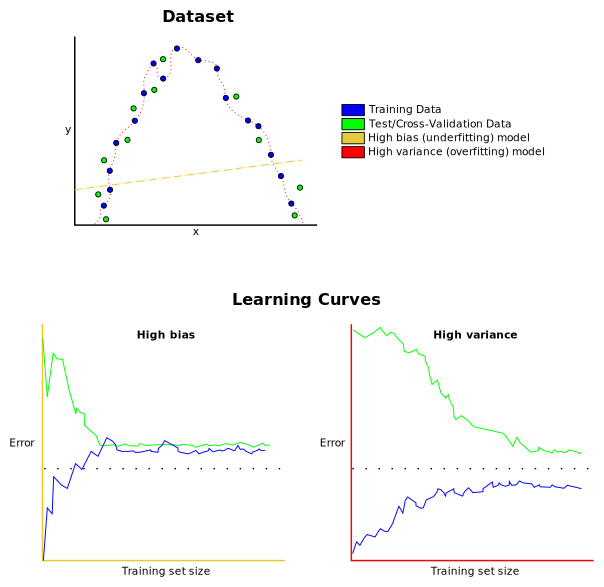
\includegraphics[width=\textwidth]{fitting.pdf}
    \caption{Plot showing a high bias (underfit) model in yellow and a high variance (overfit) model in yellow.
        Below are learning curves corresponding to each of these respectively.
        Learninv curves show the effect of different training set sizes on the training and test error of misspecified models.
        Overfitted models show a large gap between test and training errors, they fit to the training data well but don't generalise
        to new data (i.e. test data).
        Underfit models show a very high training error and little difference between test and training data as the model is too simple
        to fit the training data at all.
    }
    \label{fig:fitting}
\end{figure}



%Similar to statistics in general, approaches can be parametric or non-parametric in machine learning and can
%be easily distinguished by the change in numbers of parameters are training set size increases.
%For parametric approaches the number of parameters are fixed and finite e.g. when fitting a gaussian distribution
%to a dataset the only parameters are mean and variance of the distribution no matter how many data points are used.
%Non-parametric models on the other hand have an increasing number of parameters as the training set
%increases in size e.g. Dirichlet processes.  Typically, parametric models are faster but are less flexible as
%they make more assumptions about the dataset, whereas non-parametric approaches can be computationally infeasible
%for large datasets \citep{Bishop2006}.
%\section{Fitting}
%``Curse of dimensionality'': as the number of input/feature dimensions increase any training dataset
%will become increasingly sparse.  Parametric models are one solution to this.


Machine learning is typically divided into 2 main subsets depending on the nature of the dataset involved: 
supervised learning (e.g. classification and regression) and unsupervised learning (e.g. clustering,
density estimation and dimensionality reduction).
There are also approaches that blend features of both supervised and unsupervised learning known as semi-supervised
learning as well as an alternative idea known as reinforcement learning built on the premise of the psychology
of behaviour and the indirect reward of trial and error approaches \citep{Bishop2006}.

\subsection{Supervised Learning}

In supervised (also referred to as predictive) learning the principal aim is 
to learn a mapping between inputs/features \(x\) and outputs/response \(y\) from a set of 
inputs and their corresponding expected output.  This is known as the training set 
i.e. \(\mathcal{D} = {(x_{i}, y_{i}) \forall i \in N}\) where \(N\) is 
the cardinality of the training set \citep{Murphy2012}.  
A supervised learning algorithm thus seeks to approximate \(y=f(x)\) where \(f\) is an unknown 
function. This estimated function \(\hat{y} = \hat{f}(x)\) (see \ref{eq:sup}) would then generally
be applied to new data known as the test data for which the expected outputs are not known (i.e. 
\(x_{i} \not \in \mathcal{D}\)).

\[
    \begin{bmatrix}
        x_{0,0} & \cdots & x_{0,j}\\
        \vdots & \ddots & \vdots \\
        x_{i,0} & \cdots & x_{i,j}\\
    \end{bmatrix} \overset{\hat{f}}{\rightarrow} \begin{bmatrix}
        y_{0} \\
        \vdots \\
        y_{i} \\
    \end{bmatrix}
    \label{eq:sup}
\]

Supervised learning is further subdivided into two approaches depending on the nature of the expected
outputs: classification and regression\footnote{It is worth noting that the somewhat confusingly named
    ``logistic regression'' is typically a form of classification}.

In regression the desired outputs are real-valued (or ordinal) i.e. \(y_{i} \in \mathbb{R}\) and we seek to
estimate a particular output quantity for a specific input.
The simplest example of this would be the 2-dimensional linear regression problem mentioned above in which
we are determining the parameters of a line (gradient/weight and intercept/bias) which best fits the training 
dataset (\(\mathcal{D}\)) composed of pairs of \(x\) and \(y\) values.  Once this line has been found we 
can use it to predict the value of \(\hat{y_{i}}\) for data in the test set \(x_{i} \not \in \mathcal{D}\).


On the otherhand, in classification applications are supervised learning problem in which the expected outputs are 
categorical or nominal variables such as class labels like ``host'' and ``endosymbiont'' 
(\(y_{i} \in {host, endosymbiont, ... C}\)).  These classifications can be binary (two possible outputs i.e. 
\(y={0,1}\)), multiclass (\(\left\vert{{y}}\right\vert > 2\)),
or multi-label (similar to multiclass but outputs aren't mutually exclusive, i.e. an input can belong
to multiple classes) \citep{Murphy2012}. 


Supervised learning algorithms can additionally be either probabalistic or non-probablistic and generative or 
discriminative.
Probabilistic functions will return a probability distribution associated with possible class labels or
regression values whereas non-probablistic approaches will only return the most likely class label or value.
Continuing 
Generative algorithms, such as Naive Bayes, seek to model the process by which the output data was generated 
from the input i.e. learn the joint probability \(p(x,y)\) and make predictions on that basis via Baye's Theorem (see \ref{eq:bayes}) 

\[
    p(x,y) = p(x|y)p(x) = p(y|x)p(y)
    p(y|x) = \frac{p(x,y)}{p(y)}
    p(y|x) = \frac{p(x|y)p(y)}{p(x)}
    \label{eq:bayes}
\]

Whereas, discriminative classifiers, such as logistic regression/linear classifiers,
model the posterior probability \(p(y|x)\) directly or just learn mappings in the case of non-probabalistic approaches.
In other words, for classification problems a generative model would determine the statistical distribution of 
individual classes whereas discriminative models would just determine the boundaries between them.
Generative models often perform better on small training sets by preventing overfitting with discriminative
classifiers performing better as the training set grows \citep{Ng2002}.


%Generally, our functional approximation is probablistic - it will return the most
%probable class label \(\( \hat{f}(x) = \argmax{C} p(y = c|x,\mathcal{D}) = \hat{y}\) 
%where \(p(y|x,\mathcal{D})\) represents the probability distribution over possible labels 
%with a specific input vector \(x\) and training set \(\mathcal{D}\).
%probablistic classifiers 

\subsubsection{Support Vector Machines}

Support Vector Machines (SVMs) are a type of sparse kernel maximum-margin supervised classification algorithm.
With the innovation of the kernel trick in 1992 \citep{Boser1992} and soft-margins in 1993 (not published until \citep{Cortes1995}) SVMs have been among the most successfully applied classification algorithms throughout the 
90s and early 2000s and have only recently begun to lose ground to the resurgence of deep- and/or convolutional
neural networks e.g. \citep{LeCun1998}.  

As SVMs are a type of maximum-margin classifier this means that not only do they try to determine the parameters \(w,b\) of a hyperplane \(h_{w,b}(x) = g(w^{T}x+b)\) 


which separates two different sets of data with different class labels but that they try to find

the hyperplane which maximises this separation.  



differentiates two groups of class labels but they attempt to find a function that maximises the boundary
between the two groups.


%A function \( f: A\to B \text{where} A \text{and} B\) are any sets, the kernel or null space is defined
%by \(Ker(f) = {x: x \belongs A \text{such that} f(x) = 0}\).  The kernel is the subset of A that maps to 
%0 in the function.


Many kernel based functions are computationally infeasible on large datasets due to the combinatorial explosion
of functions which must be evaluated when every pair must be considered.

Sparse kernel methods are those that only evaluate the kernel on a subset of training points.

A major advantage of SVM are that is a true convex optimisation problem so any solution is a the global
optimum and it can't get stuck in local optima.

Only outputs decisions (i.e. labels) not label probabilities (RVM for that).




SVMs builds on the concept of a basic 2-class linear classifier i.e. learning the weights \(w\) and biases \(b\)
to return a label \(y\) for a given \(x\):
\[
    y(x) = w^{T} \phi(x) + b
\]



For linearly separable data, there will be many solutions to this as many different lines (i.e. weights and biases, aka gradient and intercept) 
can be drawn to perfectly separate the two groups of data. Therefore, the goal is then to find the line which minimises generalisation error.
In other words, the line that performs best on new data that the classifier hasn't been trained on. 

SVMs attempt to do this by maximising the distance between any samples in the training data and the decision boundary (i.e. line). 
This is known as the `margin' 





\begin{figure}[h]
    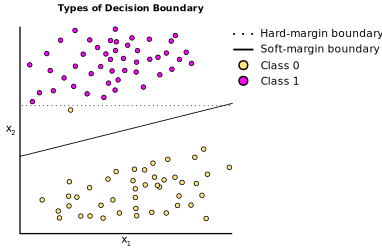
\includegraphics[width=\textwidth]{boundary.pdf}
    \caption{Demonstration of the utility of a soft-decision boundary to improve the overall
    fit of a decision boundary by allowing a degree of misclassification during training}
    \label{fig:boundary}
\end{figure}




\begin{figure}[h]
    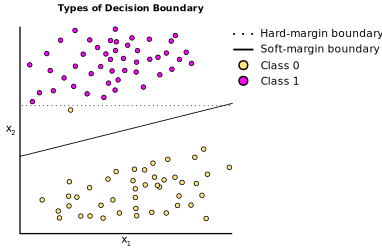
\includegraphics[width=\textwidth]{boundary.pdf}
    \caption{Demonstration of the utility of a soft-decision boundary to improve the overall
    fit of a decision boundary by allowing a degree of misclassification during training}
    \label{fig:boundary}
\end{figure}



SVMs are very good with low training datasets, and fast to classify (if not train) 






\subsection{Unsupervised Learning}

The other main form of machine learning is that of unsupervised or descriptive learning.
In which the training dataset has no provided output labels (y) i.e. 
\(\mathcal{D} = {x_{i} \forall i \in N}\) (where again N is the cardinality of 
this training dataset). In other words, we just have our dataset and have no additional information.
This is slightly more difficult problem as it lacks an obvious error metric like supervised learning 
(i.e. difference between actual output and expected output) but is important and useful tool to
try to discover patterns in datasets.

There are two major groups of unsupervised learning algorithms, the first of which is clustering algorithms
such as K-means that seeks to partition a dataset into a set of groups (see \ref{k-means} for more details).
The other major group of unsupervised algorithms are those used for visualisation and/or
dimensionality reduction.  Dimensionality reduction is a way of projecting a multidimensional
dataset into a lower number of dimensions in a way that still corresponds to
``shape'' of the data in the original number of dimensions.  

Formally, dimensionality reduction seeks to take a set of data (\(\mathcal{D}\)) and convert it
to a lower dimension form \(\mathcal{Y}\) known as a map \(\mathcal{Y} = {y_{i} \forall i \in N}\) 
with each individual \(x_{i}\) in \(\mathcal{D}\) represented by a corresponding map point \(y_{i}\). It
also seeks to do this in a way that maintains as much of the structure found in the original data 
as is possible \citep{Maaten2008} therefore, if two data points are similar in the original dimensions
they should still be similar in the map \(\mathcal{Y}\) (and the inverse).
Some dimensionality reduction approaches are well known in biology, specifically: principal component analysis (PCA) 
\citep{hotelling1933analysis} and multidimensional scaling (MDS) \citep{Torgerson1952} which both aim to identify
hidden features within the dataset that can explain a high degree of the variation.  


As ever different methodologies have a range of pros and cons, with
some better at preserving global structure (e.g. isomap) and others local data structures (e.g. local linear embedding) and so on.

One of the most recent innovations in this area is that of t-distributed stochastic neighbour-embedding
(t-SNE) in which the similarity of data points in the input space is modelled as pairwise probabilities 
using Gaussian distributions.
These probabilties are then translated into positions in the map \mathcal{Y} and similarities re-calculated
using Student's t-distributions.  The position and variance of these points and distributions respectively
is then optimised by mininising the difference between the similarity probabilities in the input space
and on the map \citep{Maaten2008}.

\subsubsection{K-means}

K-means clustering is a non-probabilistic unsupervised learning 
method in which we seek to partition data points in multidimensional space into 
K clusters. It is often used to initialise Gaussian mixture models.

Specifically, given a set of \(N\) observations \(X = {x_{1},...,x_{N}}\) 
of \(\mathcal{D}\) dimensions partition each point \((x_{n})\) into K clusters

A cluster can be intuitively considered as a group of observations/points which are 
``closer'' to one another than to other observations and the k-th cluster can 
defined by a \(\mathcal{D}\) dimensional vector \(\mu_{k}, where k=1,..,K\) for all clusters.
This vector represents the current ``prototype'' centroid of cluster. 

So, with k-means clustering we actually seek the set of K cluster centroids \({\mu_{k}}\) 
which minimise the sum of squares distances of each data point from its closest cluster centroid.
\citep{Bishop2006}

If we define a 1-of-K coding scheme with \(r_{nk} \belongs {0,1}\) as a binary variable that is 1 when \(x_{n}\) has been
assigned to cluster \(k\) (with centroid \(\mu_{k}\)) and 0 otherwise then we can define an objective cost function (\(J\)) 
that represents the sum of squares distances of each data point \(x_{n}\) from its assigned cluster centroid \(\mu_{k}\).

\[ 
    J = \sum_{n=1}^{N}\sum_{k=1}^{K} = r_{nk} \|x_{n} - \mu_{k}\|^{2}
    \label{eq:kmeans_cost}
\]

Therefore, the goal of k-means clustering is to find values for \({r_{nk}}\) and \({\mu_{k}}\) that minimise this linear 
function \ref{eq:kmeans_cost}.
\citep{Bishop2006}


The standard algorithm proceeds in two alternating steps following the initialisation of \(\mu_{k}\) with starting
cluster centroid locations \citep{Forgy1965,Lloyd1982}:
\begin{enumerate}
    \item \(\argmin_{r_{nk}} J\) i.e. minimise \ref{eq:kmeans_cost} w.r.t the assignment of points to clusters while keeping
        the cluster centroids fixed.
    \item \(\argmin_{\mu_{k}} J\) i.e. minimise \ref{eq:kmeans_cost} w.r.t the position of the cluster centroids while keeping
        the assignment of points to centroids fixed.
\end{enumerate}

Step 1 roughly corresponds to the expectation step in the expectation-maximisation (EM) algorithm and is trivially achieved by 
assigning each point to the cluster represented by the nearest centroid or formally:
\[
    r_{nk} = 
    \begin{cases}
        1,& \text{if} k=\argmin_{j} \|x_{n} - \mu_{j}\|^{2}\\
        0,& \text{otherwise}
    \end{cases}
\]

Step 2 roughtly corresponds to the maximisation step in EM is can be determined by taking the partial derivative of \(J\) w.r.t 
\(\mu_{k}\) setting it to 0 and solving for \(\mu_{k}\):
\[
    \frac{\partial J}{\partial \mu_{k}} = 2 \sum_{n=1}^{N} r_{nk} (x_{n} - \mu_{k})
    0 = 2 \sum_{n=1}^{N} r_{nk} (x_{n} - \mu_{k})
    \mu_{k} = \frac{\sum_{n} r_{nk}x_{n}}{\sum_{n} r_{nk}}
\]

In otherwords set \(\mu_{k}\) to the mean of all data points \(x_{n}\) assigned to cluster \(k\) thus k-means \citep{Bishop2006}

These two steps are repeated until a specified maximum number of iterations are reached or no points change cluster assignment during
step 1.

\(J\) \ref{eq:kmeans_cost} will converge but is liable to get stuck in a local rather than global minimum.

K-means has many modifications and improvements such as refinining the initialisation of the clusters by 
the Bradley-Fayyad method (clustering random samples of the dataset and then k-means clustering the resulting clusters) \citep{Bradley1998} 
or overclustering (running more than k-means clustering with more than the specified number of clusters and merging clusters at the end
to generate the correct number of clusters).

An efficient implementation of the k-means algorithm is available in the MLPACK C++ Machine Learning library \citep{mlpack2013}.






Disadvantages of K-means, requires a specified number of clusters (therefore diagnostics to check number of clusters)
Can converge to local optima.

Ways of specifying numbers of clusters \(k \equivalent \root{\frac{N}{2}}\) or information criteroin



\begin{figure}[h]
    \includegraphics[width=\textwidth]{knn.pdf}
    \caption{Demonstration of the KNN algorithm applying 3 rounds of Expectation-Maximisation (labelled
    1a,2a,3a, and 1b,2b,3b respectively) }
    \label{fig:knn}
\end{figure}




%\subsubsection{t-Distributed Stochastic Neighbour Embedding (t-SNE)}
%t-SNE is recently developed unsupervised visualisation/dimensionality reduction algorithm 
%created by Hinton and van der Maaten \citep{Maaten2008}
%
%t-SNE converts the high-dimensional input data \mathcal{D} into a set of probabilities that represents
%how similar each pair of points are to one another.  Specifically, a student's t-distribution
%is centered on each data point with a specified variance  
%
%Specifically, \[
%    \text{similarity of point} \(x_{i}\) \text{to} \(x_{j}\) = p_{j|i}
%    p_{j|i} = \frac{\exp{\frac{-x ||x_{i} - x_{j} ||^{2}}{2\sigma^{2}_{i}}}}{
% 
%
%
%
%Data that forms distinct groups in t-SNE but overlap in PCA indicates datasets that are not
%linearly separable but may be amenable to non-linear methods.






\section{Phylogenetics}

Phylogenetics is an effective tool with which to investigate the evolutionary 
ancestry biological sequence data, specifically DNA/RNA and protein sequences.

Phylogenetics can be used for identification of genes, species, and even populations.
Used for the estimation of evolutionary processes such as selection pressure,
migration, genome reduction, horizontal gene transfer.
Comparisons of different species/genes/populations, pin-pointing of ancestral states
and transitionary processes.



Estimation of phylogenetic trees is non-trivial as the number of possible trees
expands rapidly with the number of sequences.

For rooted phylogenies:
\begin{displaymath}
    N_{trees} = \prod_{x=2}^{N_{taxa}} (2x - 3)
\end{displaymath}



Essentially, phylogenetics is a process by which these possible trees are searched
in order to find an optimal tree according to certain criteria.




Furthermore, phylogenetic trees are important beyond just direct molecular evolution
as many biological processess can be effectively modeled in bifurcating systems
SUCH AS


% The next key method in this project is that of phylogenetics as it is an effective tool with
% which to investigate the evolutionary ancestry of the genes recovered in the transcriptome and
% to identify the likely origin (host, endosymbiont, contaminant) of these transcripts. It can also
% be used to identify potential horizontal gene transfer events between host and endosymbiont
% by searching for single gene/transcript phylogenies that have an incongruent branching pattern
% compared to established species trees. The key stages in a phylogenetic analysis are that of
% alignment (in which homologous sites in the sampled sequences are aligned with one another),
% masking (in which sites which are evolutionarily informative – can be determined to be ho-
% mologous but also non-invariant are selected), model selection (in which a sequence evolution
% model is selected using criteria such as Akaike’s information criterion which penalise increased
% parameterisation but attempt to maximise model likelihood), and finally, phylogenetic recon-
% struction (in which the selected evolutionary models are applied to the dataset using principally
% maximum-likelihood or Bayesian methodologies in order to reconstruct the likely evolutionary
% relationships in the masked sequences).

\subsection{Sequence sampling}

Bias, long branches

\subsection{Multiple Sequence Alignment}

Arguably the most important step in phylogenetics is that of multiple sequence
alignment (MSA).  The goal of MSA is to align sets sequences such that 
evolutionarily homologous residues occupy the same column. In other words,
any given column in the alignment theoretically should contain amino acid or nucleotide residues
that derive from the same common ancestor and have evolved in each sequence lineage.
It is also possible that insertion or deletion events have taken place
and a particular residue is absent in the ancestral node or a sequence lineage.

This is a non-trivial computational problem which has been proven to have an NP-complete
\footnote{A decision problem for which an answer can be verified in polynomial time 
    by a non-deterministic turing machine and to and from which any NP-hard problem
    can be translated \citep{Karp1972}.} computational complexity \citep{Wang1994}.
Specifically, the optimal alignment of N sequences has a complexity of \[ O(L^{N}) \]
for \[ N\] sequences of length \[ L \]\citep{Sievers2011}.

Due to this complexity, the majority of MSA algorithms implement heuristic approaches
in order to get, if not the optimal solution, but a sufficiently good one in a reasonable
amount of time. 

Typically, MSA algorithms start by generating the sets of all pairwise alignments. 
This alignments are all generated 

Pairwise alignment algorithms are almost all based upon a
pair of ``Ur-algorithms'' with different goals: 
Needleman-Wunsch, a global alignment algorithms (which attempt to maximise 
alignment quality over entire sequence lengths) \citep{Needleman1970} and Smith-Waterman, 
a local alignment algorithms (which are optimised towards producing high quality alignments
in sub-strings) \citep{Smith1981}.  While early, MSA algorithms were typically
largely derived from Needleman-Wunsch most modern algorithms seek to combine 
optimisation of local and global alignments 


The mostly widely heuristic used to go from a series of pair-wise alignments to
a useful MSA is that of progressive-alignment \citep{Feng1987} (implemented in 
tools such as CLUSTAL W \citep{Thompson1994}) in which the pairwise alignment
scores are built into a distance matrix summarising the relative divergence of 
each pair of sequences. From this matrix a ``guide-tree'' is generated using simple
neighbour-joining methods (in which a tree is built by recursively clustering
the least dissimilar sequences \citep{Saitou1987}).  Sequences are then progressively
aligned using their branching order within this guide-tree \citep{Thompson1994}..
This drastically reduces the \[O(L^{N})\] complexity to approximately \[O(N^{2})\]
\citep{Sievers2011}. While there have been various improvements and alternative approaches
created such as merging both local and global alignment \citep{Notredame2000}, 
rapid identification of homologous regions using Fast Fourier Transforms \citep{Katoh2002},
iterative refinement of alignments \citep{Edgar2004a} and use of Hidden-Markov Models \citep{}<++>







That is the theoretical goal of MSA, however, clearly we cannot directly observe
the ancestral state of a residue in the common ancestor of two sequence lineages.
Therefore, MSA algorithms seek to indirectly infer a homologous alignment by 
introducing gaps into sequences in order maximise
an alignment ``score'' in which matches or alignments of more frequent
substituions (e.g. Leucine and its isomer Isoleucine or Adenine to its fellow purine base
Guanine (transition)) are positively scored and gaps (extension of a gap is typically
less penalised than creating a gap) or unlikely changes (e.g. the transversion
of Adenine to Cytosine or Glutamine to Cysteine) penalised.

This will generally be codified in a substitution matrix e.g. the PAM \citep{Dayhoff1978}, 
BLOSUM \citep{Henikoff1992} amino acid matrices and their numerous subsequent
derivations and improvements. 




Using these matrices MSA algorithms will typically
align pairs of sequences and then use this set of pairwise-alignment scores
to estimate a ``guide tree''.  This guide-tree is then used to infer the order 
in which the MSA is built







 








There have been compelling arguments as early as 1991 that MSA are inherently flawed as consideration of 
evolutionary processess in the objective weighting and assessment of potential alignments \citep{Thorne1991}.
Furthermore, joint inference of alignment and phylogenetic trees minimises the risk
of conscious or subconscious research bias towards alignments and subsequent 
phylogenies that support their pre-conceived ideas.


and trees should be jointly inferred \citep{Thorne1991,Bouchard-Cote2013}

bias that alignment and inferences should be jointly estimated \citep{Redelings2005}.
While, this approach has been coded in interest probabilistic programming approaches
such as that implemented in BALI-phy \citep{Suchard2006} it is still far too
slow a process to infer phylogenies in this manner on large or even moderate datasets.
Therefore, for now independent alignment estimation is here to stay, at least until
computation resources and algorithmic development has continued until these more
theoretically satisfying approaches become feasible.

\subsection{Masking}

\subsection{Model selection}

\subsection{Phylogenetic inference}



\subsubsection{Maximum likelihood}

\subsubsection{Bayesian}







\section{OLD CRAP}
%\subsection{RNA-Seq}
%Transcriptomics and specifically RNA-Seq is one of the key investigative techniques that will be used in this project.  
%By extracting and sequencing mRNA expressed by host and endosymbiont during day and night conditions we will identify key genes involved in endosymbiotic interactions.
%RNA-seq is a second-generation sequencing technology developed to perform high-throughput short-read sequencing of cDNA generated from extracted RNA [Grabherr, 2011]. 
%As ribosomal RNA forms such a significant portion of cellular RNA it is necessary to remove it before sequencing in order to make meaningful inferences of transcript expression.  
%This can be achieved either by ribosomal depletion in which ribosomal sequences are bound by adaptors which in turn bind to magnetic beads allowing the mechanical removal of these molecules.  
%This methodology allows the preservation of smaller non-coding RNAs present in the system. However, as we are principally interested in transcripts and are operating in a eukaryotic system with poly-adenylated mRNA we can efficiently isolate mRNA via a poly-A selection, in which poly-T primers are used in reverse-transcription of mRNA into cDNA.
%From this point RNA-Seq proceeds in the same manner as other next-generation sequencing methods. 
%We are using a method known as paired-end sequencing (available on the Illumina HiSeq 2000 platform) in which 76bp reads are sequenced at either end of a 200-500bp insert. 
%This improves the ease of transcriptome assembly by providing additional positional information when producing de-Bruijn graphs. 
%
%\subsection{Transcriptome Assembly}
%Assembly is the process by which the short high-throughput sequencing reads are combined to recover the longer transcripts from which they have been randomly sampled.  
%In the simplest sense, this process relies on the quality score weighted alignment of reads.  
%Transcriptome assembly can be done in two ways: referenced (in which reads are aligned to a reference genome), and de-novo (in which the reads are assembled without a reference).  
%De-novo assembly are mainly conducted using k-mer based de-Bruijn graph creation.  
%Very briefly, reads are subdivided into k-mers (\textasciitilde $15-30$ nucleotide sequences) to aid in computation and then assembled in graphs based on k-1 overlaps between k-mers.
%With the exception of repeated regions the transcript is recovered by finding the shortest path around the graph visiting all vertexes once (i.e. a hamiltonian path). 
%In reality, assembly algorithms weight the construction of these k-mers and graphs using sequence quality scores and a large number of established heuristics.
%Referenced assemblies are often considered sub-optimal in some eukaryotic organisms due to alternative splicing and other transcript modifications not directly represented in the genomic sequences.  
%Despite this, for a \textit{Paramecium - Chlorella} transcriptome, host transcripts could still potentially be assembled as the closest available genome sequence is that of the \textit{Paramecium tetraurelia} macronuclei in which most intronic elements have been spliced out [Mayer \& Forney 1999].  
%However, using this genome as a reference for the assembly of host transcripts may be highly misleading due to the fact that this organism does not harbour \textit{Chlorella} endosymbionts and thus may lack the genes required to maintain this system and also has undergone two rounds of whole genome duplication since sharing a common ancestor with \textit{Paramecium bursaria} potentially leading to high levels of sequence divergence.  
%On the other hand, endosymbiont transcripts could be assembled using the endosymbiotic \textit{Chlorella} NC64A genome [Blanc et al., 2010] once the relationship between this organism and the endosymbiont within the CCAP 1660/12 culture is determined phylogenetically and is determined as meaningfully close.  However, the potential issue of alternative splicing would occur if we were to use this genome sequence.  
%Therefore, our initial assembly was conducted de-novo (i.e. without any reference genomes) in order to attempt to avoid biasing due to these reference genomes.   
%
%
%\subsection{Phylogenetics}
%The next key method in this project is that of phylogenetics as it is an effective tool with which to investigate the evolutionary ancestry of the genes recovered in the transcriptome and to identify the likely origin (host, endosymbiont, contaminant) of these transcripts.  
%It can also be used to identify potential horizontal gene transfer events between host and endosymbiont by searching for single gene/transcript phylogenies that have an incongruent branching pattern compared to established species trees.    
%The key stages in a phylogenetic analysis are that of alignment (in which homologous sites in the sampled sequences are aligned with one another), masking (in which sites which are evolutionarily informative – can be determined to be homologous but also non-invariant are selected), model selection (in which a sequence evolution model is selected using criteria such as Akaike's information criterion which penalise increased parameterisation but attempt to maximise model likelihood), and finally, phylogenetic reconstruction (in which the selected evolutionary models are applied to the dataset using principally maximum-likelihood or Bayesian methodologies in order to reconstruct the likely evolutionary relationships in the masked sequences). 
%
%\subsection{Annotation}
%In order to identify proteins putatively involved in endosymbiosis – namely transporters and secreted proteins and to identify proteins likely involved in their regulation it is necessary to functionally annotate assembled transcripts.  
%This was achieved in a variety of ways including Hidden-Markov Models or HMMs (via HMMer, PFAM and other similar resources), alignment (via BLAST), KEGG Ontology and Gene Ontology annotation (via tools such as the KEGG Automated Annotation Server or BLAST2Go). 
%HMMs are a commonly used tool in sequence identification and depending on their training are generally more sensitive than alignment based methods [Eddy., 2011].
%This will be further discussed within the methods.
%
%\section{Methods}
%\subsection{Culturing}
%
%\subsection{RNA-Seq}
%\subsubsection{cDNA generation and library preparation}
%
%Purified RNA from day and night samples were pooled into a single day and a single night sample due to limitations on the quantity of extracted RNA. 
%These two samples were then prepared for sequencing using the TruSeq Stranded RNA preparation kit (Illumina).  
%mRNA was selected using a poly-A selection method before being fragmented, cleaned-up using ethanol and then reverse transcribed into single-stranded cDNA using random hexamer primers. 
%The prepared ds cDNA was then end-repaired or cleaved to produce blunt-ended fragments.  
%By the addition of a trailing A-base to these fragments sequencing adaptors were added using an overlapping complementary T-base.  
%Fragments were then denatured and amplified before cluster generation using the standard Illumina sequence library preparation methods [\url{http://res.illumina.com/documents/products/datasheets/datasheet_truseq_sample_prep_kits.pdf}].
%
%\subsubsection{Sequencing}
%
%Clonal cluster generation by bridge amplification was conducted on the cBot (Illumina) platform using the TruSeq Paired-End cluster kit (Illumina).  
%The samples were run in individual lanes on a HiSeq 2000 8-lane flow-cell (Illumina) to produce 76bp paired-end reads. 
%Sequencing was conducted at the University of Exeter sequencing service.
%
%\subsubsection{Assembly}
%The paired-end fastq reads from the sequencing experiment were trimmed to sequences of sufficient quality and sequencing adaptors removed. 
%Reads from day-and-night runs were assembled separately as well as a combined assembly of all the reads. 
%As the \textit{Paramecium bursaria} 1660 genome or the \textit{Chlorella} endosymbiont (CCAP12) have not yet been sequenced de-novo transcriptome assembly was conducted (further explanation for this in background section).  
%This was done using both the Oases package [Schluz, 2012] from European Bioinformatics Institute [\url{http://www.ebi.ac.uk/~zerbino/oases/}] and the Trinity package [Haas, 2013] provided by the Broad Institute [\url{http://trinityrnaseq.sourceforge.net/}] using a high-memory computing cluster at the University of Exeter.  
%Assemblies were compared and a single assembly methodology was selected for further downstream analysis. 
%
%\subsubsection{Saturation}
%In order to assess whether increased sequencing depth would recover further transcripts a read-saturation analysis was conducted.  
%This was achieved by developing a program to repeatedly take random subsamples of the paired-end reads (from the day sample, the night sample and the combined pool) and assessing the number of the assembled transcripts that could be successfully recovered using these reads.  
%This was done with the aid of a short-read aligner bowtie-2 [Langmead, 2012], standard GNU/Linux command line tools, and a custom python script.  
%The results were plotted using python+matplotlib and assessed for saturation in transcript recovery
%
%\subsubsection{Extracting Likely Coding Regions}
%As host and endosymbiont use different codon tables it was necessary to identify ORFs in the assembled transcripts using both tetrahymena (i.e. Host/Paramecium) and universal (endosymbiont/Chlorella and bacterial contaminant/foodstock) encodings.  
%The ciliate `tetrahymena' encoding differs from universal codon look up tables in that UAA and UAG which are normally stop codons instead code for glutamine, this means \textit{Paramecium} only has a single stop codon (UGA) [Harper \& Jahn, 1989].
%This was conducted using the Trinity transcripts\_to\_best\_scoring\_ORFs tool [\url{http://trinityrnaseq.sourceforge.net/analysis/extract_proteins_from_trinity_transcripts.html}].  
%Initially, this tool identifies the longest ORF within each assembled transcript.  
%These longest ORFs are used to train a hexamer-based HMM which is then used to identify the ORFs with highest likelihood.  
%These ORFs are then translated into peptide sequences. 
%
%\subsubsection{Transcript Identification}
%Despite care being taken in filtering and washing-off bacteria from the \textit{Paramecium} prey food-stock and usage of poly-A selection, bacterial contamination was still present in our assembled contigs.  
%Therefore, it was necessary to develop a pipeline to identify the transcript origins to filter those transcripts originating from host and endosymbiont. 
%Initially transcripts were binned into their predicted source - Host (H), Unknown but likely Host (U(H)), Endosymbiont (E), Unknown but likely Endosymbiont (U(E)), Food (F), Unknown but likely Food (U(F)), and Unknown (U).  
%Each of the assembled transcripts were BLASTed against a database consisting of the following genomes: \textit{Chlorella} NC64A, \textit{Chlamydomonas reinhardtii}, \textit{Coccomyxa} C169, \textit{Paramecium tetraurelia}, \textit{Tetrahymena thermophila},  \textit{Arabidopsis thaliana}, \textit{Homo sapiens} (helping to identify contamination), \textit{Saccharomyces cerevisiae}, \textit{Schizosaccharomyces pombe}, \textit{Bacillus cereus} ATCC 14579, \textit{Escherichia coli} 536, \textit{Escherichia coli} O157 H-7, \textit{Salmonella typhimurium} LT2 and \textit{Escherichia coli} K-12 (the last 5 genome datasets helping to identify food bacterial genes).  
%The bins were classified as follows:
%\begin{itemize}
%  \item Endosymbiont (E): Transcript's highest scoring BLAST hit at -50E was to \textit{Coccomyxa}, \textit{Chlamydomonas} or \textit{Chlorella}.  Or transcript's highest scoring hit at -20E was one of those species and the longest likely coding region in the transcript was using the universal codon table. 
%  \item Unknown but likely Endosymbiont (U(E)): -10E hit to \textit{Coccomyxa}, \textit{Chlamydomonas} or \textit{Chlorella} and longest likely coding region was using the universal codon table. Or transcript's highest hits at -10E and -20E were to one of those genomes regardless of coding region presence.
%  \item Host (H): Transcript's highest hits at -50E were to \textit{Paramecium tetraurelia} or \textit{Tetrahymena thermophila}.  Or highest hit at -20E was one of those species and longest likely coding region was using the Tetrahymena codon table.
%  \item Unknown but likely Host (U(H)): -10E hit to \textit{Paramecium tetraurelia} or \textit{Tetrahymena thermophila} and longest likely coding region was was using the Tetrahymena codon table. Or transcript's highest hits at -10E and -20E were to one of those genomes regardless of coding region presence.
%  \item Food (F): Transcript's highest scoring BLAST hit at -50E was to one of the \textit{E. coli} species or \textit{Salmonella}.  Or transcript's highest scoring hit at -20E was one of those species and the longest likely coding region in the transcript was using the universal codon table.
%  \item Unknown but likely Food (U(F)): -10E hit to one of the \textit{E. coli} species or \textit{Salmonella} and longest likely coding region was using the universal codon table. Or transcript's highest hits at -10E and -20E were to one of those genomes regardless of coding region presence.
%  \item Unknown (U): highest scoring hits to \textit{Arabidopsis}, \textit{Homo sapiens}, \textit{Saccharomyces} or \textit{Schizosaccharomyces} or any sequence not fitting into the above categories.
%\end{itemize}
%
%In order to assess the accuracy of the `binning' of endosymbiont sequences and to estimate how many host or endosymbiont transcripts we would accidentally discard using these categories we used a phylogenetic analysis pipeline to verify the likely ancestry and therefore point of origin within the endosymbiosis of each sequence.  
%A script was created used the translated transcript peptide sequences to search a database of over 900 representative genomes using BLASTp.  This script recovered all sequences above an E-value of $10^{-5}$. 
%These sequences were then automatically aligned and masked using MUSCLE [Edgar, 2004] and TrimAL [Capella-Gutierrez, 2009]. 
%Fast maximum-likelihood trees were then generated for each masked alignment using FASTREE2 program [Price, 2010].  
%These trees were then converted to scalable vector graphics and using the NCBI taxonomy API each branch was colour coded depending on taxonomic group.  
%This allowed for quick manual inspection to determine the likely origin identity of the initial transcript.  
%For example, if a transcript sequence was found to branch largely within archaeplastida species it was considered as likely originating from the endosymbiont.  
%Likewise, if it branched largely among ciliate species it was considered as likely host-derived.  
%Continuing in the same vein, those sequences considered as being derived from bacterial food-stocks were considered as those that branched largely within bacterial clades and those sequences that branched with no clear pattern were considered to be `Unknown'.  
%Any transcripts where endosymbiont sequences were found to branch incongruently with accepted topologies (especially within the ciliate or bacteria) were determined to be showing signs of potential horizontal gene transfers and were recorded for further analysis.  
%For example, if a transcript branched with another endosymbiotic algae (particularly \textit{Chlorella} NC64A) within a clade of ciliates this would be considered a potential HGT event to be further investigated.
%The entire initial `Endosymbiont Bin' (2,825 transcripts), the `Unknown but likely Endosymbiont Bin' (600) and the `Unknown Bin' (2,096) were phylogenetically tested using this pipeline.  
%However, owing to the size of the initial `Food Bin' (5,129) and `Host Bin' (27,907) it wasn't possible to exhaustively test all transcripts in these two bins therefore 2000 transcripts were randomly selected from each them and tested using the pipeline. 
%In the cases where too few sequences were recovered to produce a phylogeny (<3 including seed) the source proteomes of the sequences that were recovered were assessed. For example, if the recovered sequences were from the archaeplastida that was considered sufficient evidence to class that transcript as belonging to that `Endosymbiont Bin' and so on.  If no other sequences were recovered using BLASTp then the transcript was placed into the `Unknown Bin'.
%The change in initial binning after phylogenetic verification were then plotted using python+matplotlib and an estimate for the numbers of unidentified endosymbiont transcripts was made.
%
%\subsubsection{Identification of putative secreted and putative transporter proteins}
%Initial transcript functional annotation was conducted via BLAST and mapping Gene Ontology terms using the Blast2GO application [Conesa, A. et al., 2005] [\url{http://www.blast2go.com/b2ghome}].  
%In order to more accurately identify the likely proteins involved in the maintenance of the \textit{Paramecium-Chlorella} photosynthetic endosymbiosis we attempted to identify all transporter and secreted proteins within the verified endosymbiont and host transcript complements. A permissive set and conservative subset of host and endosymbiont transporter and secreted proteins were identified using a combination of pipelines.
% Putative transporter proteins were identified as all coding sequences within each bin containing 1 or more transmembrane domains (as identified by the HMM implemented in the program tmhmm 2.0c  [Krogh et al., 2001, Sonnhammer et al., 1998]).  
%The conservative subset of transporter proteins were those identified as containing 4 or more TM domains.  
%The predicted host and endosymbiont secretome was determined by combining the outputs of several established and widely-published programs for identification of secreted proteins - SignalP 4.1 [Petersen et al., 2011], tmhmm 2.0c, TargetP 1.1 [Emanuelsson et al., 2000], and WoLFPSORT 0.2 [Horton et al., 2007] (with the assistance of some accessory scripts from from UCSC [\url{http://hgdownload.cse.ucsc.edu/admin/exe/}] and the FASTX-toolkit [\url{http://hannonlab.cshl.edu/fastx_toolkit/index.html}]). 
%Input sequences were checked for the presence of N-terminal signal peptides primarily via the detection of signal peptide cleavage sites by the HMM implemented in SignalP 4.1. 
%Mature peptides (i.e. those with the detected signal peptide cleaved) output from SignalP 4.1 were then processed in tmhmm 2.0c to detect and remove any sequences containing transmembrane domains. 
%The output from these two stages were then combined with all initial input sequences detected as secreted (S) by TargetP 1.1 and as having an extracellular localisation via WoLFPSORT 0.2 to produce a single fasta formatted output file containing the entire predicted secretome, i.e. a set of proteins predicted to be secreted by all three bioinformatic methods. 
%This therefore identified the conservative subset of host and endosymbiont secreted proteins. 
%A second list of putative secreted proteins was identified as any protein predicted to be secreted by any one of either SignalP 4.1, WoLFPSORT 0.2, or TargetP 1.1. It must be noted that such prediction approaches are only as good as the quality of each individual transcript assembly. 
%Genes with low transcript levels are likely to have low coverage and assembly quality potentially leading to false negative detection of N-terminal signal peptides. 
%This was investigated in more detail below.
%
%\subsubsection{Coverage}
%As the identification of the secreted proteins hinged upon the recovery and accurate prediction of N-terminal signal peptides it was necessary to assess the position-specific read coverage across the transcript specifically at the C- and N- termini. 
%This was achieved by developing a script to count and average (median) the number of reads aligning to each nucleotide in both tetrahymena and universal (i.e. host and endosymbiont) likely coding regions using a custom python script.  
%This was done for all tetrahymena and universal coding regions in transcripts, all phylogenetically confirmed host and endosymbiont binned sequences, conservatively and permissively identified putative secreted and transporter proteins in the `Host Bin' and `Endosymbiont Bin'. 
%Results were then plotted using python+matplotlib.
%
%\subsubsection{Endosymbiont Species Confirmation}
%In order to confirm the identity of the endosymbiont species from CCAP two analyses were conducted. 
%Firstly, the endosymbiont binned transcripts were searched for any 18S rRNA sequences present in the transcriptome.  
%The two identified fragments of 18S sequence were aligned against a database of green algal 18S sequences (from [Hoshina and Imamura, 2008]) using MUSCLE.    
%The multiple-sequence alignments were then masked manually using Seaview [Gouy, 2010].  
%Evolutionary model was estimated using Prottest3 [Dariba, 2011] for each masked alignment and as highest likelihood models were identical (LG+$\Gamma$+I) alignments were concatenated into a single masked alignment.  
%Bayesian and Maximum Likelihood phylogenetic reconstructions were then conducted using an un-partitioned suggested model and both MrBayes v3 and PhyML [Guindon, 2010].  
%The ML phylogeny was plotted as an SVG and key taxa were highlighted.
%
%Secondly, \textit{Chlorella} specific primers were used to amplify, clone and sequence the identifying ITS2 region.  
%This was achieved by using the Qiagen DNeasy Plant DNA extraction kit after bead beating to disrupt the \textit{Chlorella} cells from a culture aliquot. 
%Using \textit{Chlorella} specific primers (from [Hoshina and Imamura, 2008]) PCR was used to amplify the \textit{Chlorella} ITS2 region from the  extracted DNA samples.  
%These extracted samples were then sub-cloned using the StrataClone-TA-cloning kit (StrataClone) and blue-white screened for successful insert ligation. 
%9 white colonies were selected and prepared for sequencing using the SV Wizard MiniPrep kit and PCR ligation of M13 universal sequencing primers.  
%Sequences were then Sanger sequenced via Beckman-Coulter Sequencing Service.  
%The returned sequences were then used to reconstruct a phylogeny of ITS2 region using BLAST against species outlined by [Hoshina and Imamura, 2008], aligned using MUSCLE, masked in Seaview, model testing in Prottest3 and reconstructed using MrBayes and PhyML.
%
%\section{Results}
%\subsection{RNA-Seq Assembly}
%The comparison of De-novo transcriptome assemblies can be seen in assembly summary below.
%The metrics clearly show the Trinity assembly is far superior to that of the Oases assembly with over a 50\% reduction in total contig number while recovering consistently longer contigs (a histogram of the Trinity contigs lengths and distribution can be see in contig lengths). 
%All further analyses were done using Trinity based pooled assembly.
%
%\begin{table}
%\centering
%\begin{tabular}{| c || c | c |}
%\hline
%\textbf{Assembly Metric} & \textbf{Oases Assembly} & \textbf{Trinity Assembly} \\
%\hline
%\textbf{Min Contig Length:} & 100 & 201\\
%\textbf{Max Contig Length:} & 16,202 & 17,729\\
%\textbf{Mean Contig Length:} & 648.90 & 959.32\\
%\textbf{Standard Deviation of Contig Length:} & 939.04 & 1080\\
%\textbf{N50 Contig Length:} & 1,368 & 1,621 \\
%\textbf{Number of Contigs:} & 117,570 & 48,003\\
%\textbf{Number of Contigs >=1kb:} & 22,225 & 14,774\\
%\textbf{Number of Contigs in N50:} & 14,977 & 8,060\\
%\textbf{Number of Bases in All Contigs:} & 76,290,606 & 46,050,097\\
%\textbf{Number of Bases in All Contigs >=1kb:} & 46,695,005 & 31,602,626\\
%\textbf{GC Content of Contigs:} & 28.99\% & 30.97\% \\
%\hline
%\end{tabular}
%
%\caption{Pooled read RNA-Seq De-Novo Assembly Comparison}
%\label{tab:assembly_summary}
%\end{table}
%
%The saturation analysis (in which we test whether further sequencing depth would recover more transcripts) is shown in saturation.  
%As can be seen the combined reads quickly trend to an asymptote suggesting the majority of transcripts were recovered at this sequencing depth.
%
%\subsection{Transcript Analysis}
%The initial identification and binning of recovered transcripts into host and endosymbiont categories was tested using a phylogenetic approach. 
%The results of this analysis were plotted in phylogenetic confirmation.  
%This demonstrates that the initial bin identifications were accurate for endosymbiont (\textasciitilde92\%) and food ( \textasciitilde94\%) derived transcripts.  
%Of the bins that were too large to be comprehensively phylogenetically tested (`Host Bin' and `Food Bin') we screened a subset of 2000 transcripts using a phylogenomic approach. 
%There were almost no detected endosymbiont sequences in 2000 randomly selected `Food Bin' transcripts therefore the `Host Bin' was the only cause for concern in containing misidentified endosymbiont transcripts.  
%\textasciitilde 2\% of the 2000 randomly sampled `Host Bin' transcripts were found to be wrongly identified endosymbiont sequences, assuming this random sample is representative of the `Host Bin' in general this suggests approximately 500 endosymbiont transcripts are misidentified as host sequences (within the 27,907 host sequences).  
%A key result here is that the bins that are to be discarded as contaminants (i.e. `Food Bin' and `Unknown Bin') have been either exhaustively checked and all host or endosymbiont transcripts they contain recovered or, as in the case of the `Food Bin', there are minimal sequences to be found.  
%This, combined with the saturation analysis allows us to be confident that we have recovered the maximum possible (even if \textasciitilde 500 endosymbiont are misidentified as Host) host and endosymbiont expressed transcripts during day and night conditions.
%
%In order to assess the accuracy of secretome predictions it was necessary to assess terminal coverage of likely coding regions.  
%The median coverage is plotted in coverage.  The key concern that this plot raises is that of poor terminal coverage throughout the `Host Bin' and `Endosymbiont Bin'. 
%As expected the identified secreted proteins (as these predictions largely hinge on detection of terminal signalling peptides) demonstrate a greater coverage suggesting on average only those transcripts with high terminal coverage were identifiable as secreted.  
%Due to the general low level of terminal coverage in the bins as a whole this raises the distinct possibility that many secreted proteins are undetected in the `Host Bin' and `Endosymbiont Bin'. 
%Transporter proteins are principally identified by the presence of trans-membrane domains so terminal coverage is not a concern for their identification. 
%For this reason, we are initially focusing on transporter proteins, however, there is a possibility to investigate secreted proteins using alternative strategies, in particular, proteomics.  
%Mass-spectrometry based proteomics may allow the identification (via peptide fingerprinting) of secreted proteins.
%
%\subsection{Preliminary Metabolic Mapping}
%Using the KEGG Automated Annotated Server KEGG Ontology annotations were recovered for the phylogenetically verified host and endosymbiont sequences and plotted onto the KEGG complete metabolic pathway (see metabolic mapping).  This is a rough preliminary tool that we can use to target later regulatory and interaction investigations for our candidate proteins.
%
%\subsection{Endosymbiont Species Confirmation}
%
%The phylogeny generated using detected Chlorella 18S sequences (see phylogeny) within the transcriptome clearly shows the concatenated sequence branching with high basal support (99.1\%) among the clade containing \textit{Chlorella} NC64A and endosymbionts 10 and 12. 
%The concatenated sequences branch directly (with low support) with \textit{Chlorella} 12 endosymbiont as expected from the CCAP provided \textit{Paramecium bursaria – Chlorella} CCAP 1660/12 culture.  
%ITS2 sequencing is still to be completed and thus this phylogeny cannot be reconstructed at this time, this will be completed within 2 months.
%Regardless, preliminary results support the identity of the endosymbiont as being the \textit{Paramecium bursaria} CCAP 1660/12 endosymbiont and the immediate sister to \textit{Chlorella} NC64A.  This piece of data is particularly important as \textit{Chlorella} NC64A has a complete published genome sequence [Blanc et al., 2010]. As NC64A strain is both endosymbiotic and a close-relative it may form a useful resource in annotating and further exploring the assembled transcriptomic data.  
%Potentially, this genome sequence may even be used for a referenced transcriptome assembly and allow improvement in assembled transcript quality.
%
%
%\section{Progress so far}
%\begin{itemize}
%  \item Verified the taxonomic identity of \textit{Chlorella} endosymbiont within \textit{Paramecium bursaria} sample provided by CCAP using molecular phylogenetics.
%  \item Cultured and purified transcripts from \textit{Paramecium-Chlorella} system in the two key metabolic states in their relationship – active and inactive photosynthesis during lit and dark conditions
%  \item Conducted a de-novo transcriptome assembly of the day/night transcripts
%  \item Assessed assembly quality and, in particular, average terminal coverage to determine the relative quality of annotation methods.
%  \item Phylogenomically identified host and endosymbiont transcripts, as well as filtering out those derived from contaminants such as bacterial food-stocks.
%  \item Annotated extracted transcripts with a focus on transporters and secreted proteins
%  \item Generated a guide-line differential expression analysis to help target further work
%  \item Assembled preliminary metabolic network of host and endosymbiont transcripts
%  \item Identified a set of transporters putatively involved in maintenance of endosymbiosis
%  \item Begun design of antibodies to determine the localisation of these transporters
%\end{itemize}
%
%
%\section{Further Work}
%The work conducted so far forms the ground-work necessary in order make meaningful insights into possible proteins involved in the maintenance of the endosymbiosis.
%Namely, confirmation of the endosymbiont species, day and night transcriptome sequencing and assembly, identification and verification of host and endosymbiont transcripts from the transcriptome and identification of transporter and secreted proteins within these subsets.  
%Using these greatly reduced numbers of sequences it is possible to manually identify candidates to further investigate, to ideally identify their role in maintaining the endosymbiosis.  
%Once we have developed our shortlist of candidates further we hope to verify our predictions using a variety of molecular methodologies:
%\begin{itemize}
%  \item Localisation - Polyclonal antibodies to confirm candidate is able to have a direct role in endosymbiosis (localised to perialgal vacuole or endosymbiont membrane for example) within the next 6 months.
%  \item Proteomics - Shotgun Mass Spectrometry - confirm presence of protein in system rather than just transcripts within 9 months.
%  \item Differential Expression Analysis - qPCR - to verify the regulation of candidate proteins at various points in the endosymbiosis (e.g. establishment, day, night) within the next 3-6 months.
%  \item RNAi - direct testing of predictions by determining the effect of candidate protein knock-out on state of endosymbiosis within 9 months.
%\end{itemize}
%
%\section{References}
%
%\noindent Achilles-Day, Undine E M,  Day, John G Isolation of clonal cultures of endosymbiotic green algae from their ciliate hosts, 2012 Journal of microbiological methods,  92,  3, 355, 7
%
% 
%\noindent Beijirnick, M. W. 1890 Kulturversuche mit Zoolchlorellen, Lichengonidien, und anderen Algen. Botan. Zeit., Jahrg. 48].   MISSING
%
% 
%\noindent Berger J  Feeding behavior of Didinium nasutum on Paramecium bursaria with normal or apochlorotic zoochlorellae 1980 . J Gen Microbiol 118 : 397 – 404
%
% 
%\noindent Chen, Tze-Tuan, Polyploidy in Paramecium bursaria, 1940,Genentics,  26(1)
%
% 
%\noindent Blanc G, Duncan G, Agarkova I, Borodovsky M, Gurnon J, Kuo A, Lindquist E, Lucas S, Pangilinan J, Polle J The Chlorella variabilis NC64A genome reveals adaptation to photosymbiosis, coevolution with viruses, and cryptic sex. 2010 Plant Cell 22(9):2943–2955
%
% 
%\noindent Darriba D, Taboada GL, Doallo R, Posada D. Prottest3: Fast selection of best-fit models of protein evolution. Bioinformatics, 27:1164-1165, 2011
%
% 
%\noindent Dolan, John, Mixotrophy in Ciliates: A Review of Chlorella Symbiosis and Chloroplast Retention, 1992,  Marine Microbial Food Webs,  6(2)
%
% 
%\noindent Edgar, R.C MUSCLE: multiple sequence alignment with high accuracy and high throughput, 2004, Nucleic Acids Res. 32(5):1792-1797 
%
% 
%\noindent Eddy, S.R., Accelerated Profile HMM Searches, 2011, PLoS Comp. Biol.
%
% 
%\noindent Emanuelsson, O., Nielsen, H., Brunak, S., von Heijne, G., Predicting subcellular localization of proteins based on their N-terminal amino acid sequence. J. Mol. Biol.,2000. 300: 1005-1016,
%
% 
%\noindent Fujishima, Masahiro,  Kodama, Yuuki, Endosymbionts in paramecium, 2012, European journal of protistology, 48,2
%
% 
%\noindent Gouy M., Guindon S. \& Gascuel O. (2010) SeaView version 4 : a multiplatform graphical user interface for sequence alignment and phylogenetic tree building. Molecular Biology and Evolution 27(2):221-224.
%
% 
%\noindent Guindon S., Dufayard J.F., Lefort V., Anisimova M., Hordijk W., Gascuel O. "New Algorithms and Methods to Estimate Maximum-Likelihood Phylogenies: Assessing the Performance of PhyML 3.0." Systematic Biology, 59(3):307-21, 2010.
%
% 
%\noindent Krogh A., Larsson B., von Heijne G., Sonnhammer EL., Predicting transmembrane protein topology with a hidden Markov model: application to complete genomes. J Mol Biol. 2001 Jan 19;305(3): 567-80.
%
% 
%\noindent Haas et al., De novo transcript sequence reconstruction from RNA-seq using the Trinity platform for reference generation and analysis, Nat. Protocols 2013 XXX
%
% 
%\noindent Harper, D.S., Jahn, C.L. Differential use of termination codons in ciliated protozoa 1989, PNAS, Vol. 86, pp. 3252-3256, XX
%
% 
%\noindent Horton, P., Park, K-J., Obayashi, T., Fujita, N., Harada, H., Adams-Collier, CJ., Nakai, K., WoLF PSORT: protein localization predictor Nucl. Acids Res. 2007 35 suppl 2: 585-587
%
% 
%\noindent A. Conesa, S. Götz, J. M. Garcia-Gomez, J. Terol, M. Talon and M. Robles. "Blast2GO: a universal tool for annotation, visualization and analysis in functional genomics research", Bioinformatics, Vol. 21, September, 2005, pp. 3674-3676.
%
% 
%\noindent Hoshina, R., Imamura, N,  Multiple Origins of the Symbioses in Paramecium bursaria 2008 Protist, vol. 159, 53-63
%
% 
%\noindent Hoshina, R., Imamura N., Origins of algal symbions in Paramecium Bursaria 2009, Microbiology Monographs 12 Endosymbtions in Paramecium (ed: Fujishima M.)
%
% 
%\noindent Hosoya, Hiroshi,  Kimura, Kouki, Matsuda, Seiji, Kitaura, Miyuki,  Takahashi, Tadao, Kosaka, Toshikazu, Symbiotic Algae-free Strains of The Green Paramecium Paramecium bursaria produced by the Herbicide Paraquat, 1995, Zoological Science, 12
%
% 
%\noindent Johnson, Matthew D,  Acquired phototrophy in ciliates: a review of cellular interactions and structural adaptations , 2011, The Journal of eukaryotic microbiology, 58(3)
%
% 
%\noindent Karakashian, S.J., Growth of Paramecium bursaria as Influenced by the Presence of Algal Symbionts, 1963,  Physiological Zoology, 36(1)
%
% 
%\noindent Karkashian, S.J.,  Karkashian, M.W., Evolution and Symbiosis in the Genus Chlorella and Related Algae, 1965, Evolution,  19(3)
%
% 
%\noindent Kato Y, Imamura, N. Metabolic Control Between the Symbiotic Chlorella and the Host Paramecium, 2009,  Microbiology Monographs 12,  Endosymbionts in Paramecium
%
% 
%\noindent Kodama, Yuuki, Nakahara, Miho, Fujishima, Masahiro,  Symbiotic alga Chlorella vulgaris of the ciliate Paramecium bursaria shows temporary resistance to host lysosomal enzymes during the early infection process, 2007, Protoplasma, 230(1,2)
%
% 
%\noindent Kodama, Yuuki, Fujishima, Masahiro, Infection of Paramecium bursaria by Symbiotic Chlorella Species, 2009, Microbiology Monographs 12,  Infection of Paramecium bursaria by Symbiotic Chlorella Species
%
% 
%\noindent Kodama, Y, Fujishima, M,  Induction of secondary symbiosis between the ciliate Paramecium and the green alga Chlorella 2010,  Current Research, Technology and Education Topics in Applied Microbiology and Microbial Biotechnology
%
% 
%\noindent Kodama, Yuuki, Inouye, Isao,  Fujishima, Masahiro, Symbiotic Chlorella vulgaris of the ciliate Paramecium bursaria plays an important role in maintaining perialgal vacuole membrane functions, 2011, Protist, 162(2)
%
% 
%\noindent Kadono T , Kawano T , Hosoya H , and Kosaka T (2004) Flow cytometric studies of the host-regu- lated cell cycle in algae symbiotic with green paramecium . Protoplasma 223 : 133 – 141
%
% 
%\noindent Kodama, Yuuki, Fujishima, Masahiro, Endosymbiosis of Chlorella species to the ciliate Paramecium bursaria alters the distribution of the host's trichocysts beneath the host cell cortex.2011, Protoplasma, 248(2)
%
% 
%\noindent Kodama, Yuuki,  Fujishima, Masahiro, Characteristics of the digestive vacuole membrane of the alga-bearing ciliate Paramecium bursaria , 2012  Protist 163(4)
%
% 
%\noindent Langmead B, Salzberg S. Fast gapped-read alignment with Bowtie 2. Nature Methods. 2012, 9:357-359.
%
% 
%\noindent Loefer,J. B., Bacteria free cultures of Paramecium bursaria and concentrations of the medium as a factor in growth. 1936 J. Exp. Zoo!., 72: 387
%
% 
%\noindent Mayer, K.M., Forney J.D., A Mutation in the Flanking 5'-TA-3' Dinucleotide Prevents Excision of an Internal Eliminated Sequence From the Paramecium tetraurelia Genome 1999 genetics vol. 151 no. 2 597-604
%
% 
%\noindent Miwa I., Regulation of Circadian Rhythms of Paramecium bursaria by Symbiotic Chlorella Species 2009, Microbiology Monographs 12, Endosymbions in Paramecium.
%
% 
%\noindent Meier, Renate, Wiessner, Wolfgang, Infection of algae-free Pammecium bursaria with symbiotic Chlorella sp. isolated from green paramecia, 1989, Journal of cell science, 93
%
% 
%\noindent{} Muscatine L Glycerol excretion by symbiotic algae from corals and Tridacna and its control by the host 1967  Science 156 : 516 – 519
%
% 
%\noindent Nishihara, N, Horiike, S,  Takahashi, T, Kosaka, T, Shigenaka, Y, Hosoya, H, Cloning and characterization of endosymbiotic algae isolated from Paramecium bursaria 1998, Protoplasma, 203
%
% 
%\noindent Parker, Raymond C, Symbiosis in Paramecium bursaria, 1926, Journal of Experimental Zoology,  46
%
% 
%\noindent Pérez MT , Dolan JR , Fukai E (1997) Planktonic oligotrich ciliates in the NW Mediterranean growth rates and consumption by copepods . Mar Ecol Prog Ser 155 : 89 – 101
%
% 
%\noindent Petersen, TN., Soren, B., von Heijne, G., Nielsen, H., SignalP 4.0: discriminating signal peptides from transmembrane regions. Nat Meth 2011; 8(10):785-786
%
% 
%\noindent Price, M.N., Dehal, P.S., and Arkin, A.P. FastTree 2 -- Approximately Maximum-Likelihood Trees for Large Alignments. 2010 PLoS ONE, 5(3):e9490.
%
% 
%\noindent Putt M Abundance, chlorophyll content and photosynthetic rates of clliates in the Nordic Seds during summer.1990  Deep-Sea Res 37:1713-1731
%
% 
%\noindent Raven JA Phagotrophy in phototrophs 1997 Limnol Oceanography 42:198–205
%
% 
%\noindent Reisser W  The metabolic interactions between Paramecium bursaria Ehrbg. and Chlorella spec. in the Paramecium bursaria -symbiosis III. The influence of different CO2 concentrations and of glucose on the photosynthetic and respiratory capacity of the symbiotic unit  1980. Arch Microbiol 125 : 291 – 293
%
% 
%\noindent Salvador Capella-Gutierrez; Jose M. Silla-Martinez; Toni Gabaldon. trimAl: a tool for automated alignment trimming in large-scale phylogenetic analyses. Bioinformatics 2009 25: 1972-1973.
%
% 
%\noindent M.H. Schulz, D.R. Zerbino, M. Vingron and Ewan Birney. Oases: Robust de novo RNA-seq assembly across the dynamic range of expression levels. Bioinformatics, 2012. DOI: 10.1093/bioinformatics/bts094.
%
% 
%\noindent Sonnhammer, EL, von Heijne, G., Krogh, A., A hidden Markov model for predicting transmembrane helices in protein sequences. Proc Int Conf Intell Syst Mol Biol 1998;6:175-82
%
% 
%\noindent Sommaruga, R., Sonntag, B., Photobiological Aspects of the Mutualistic Association Between Paramecium bursaria and Chlorella 2009, Microbiological Monographs 12, Endosymbionts in Paramecium
%
% 
%\noindent Summerer, Monika, Sonntag, Bettina,  Sommaruga, Ruben,  An experimental test of the symbiosis specificity between the ciliate Paramecium bursaria and strains of the unicellular green alga Chlorella., 2007,  Environmental microbiology, 9(8)
%
% 
%\noindent Summerer, Monika, Sonntag, Bettina, Hörtnagl, Paul, Sommaruga, Ruben, Symbiotic ciliates receive protection against UV damage from their algae: a test with Paramecium bursaria and Chlorella. 2009,  Protist, 160(2)
%
% 
%\noindent Taguchi, K, Hirota, S, Nakayama, H, Kunugihara, D, Mihara, Y - Optical Manipulation of Symbiotic Chlorella in Paramecium Bursaria Using a Fiber Axicon Microlens, 2012, Journal of Physics: Conference Series, 352
%
% 
%\noindent Takeda H , Sekiguchi T , Nunokawa S , Usuki I (1998) Species-specificity of Chlorella for estab- lishment of symbiotic association with Paramecium bursaria . Does infectivity depend upon sugar components of the cell wall? Eur J Protistol 34 : 133 – 137
%
% 
%\noindent Takahashi T , Shirai Y , Kosaka T , Hosoya H (2007) Arrest of cytoplasmic streaming induces algal proliferation in green paramecia . PLoS ONE 2 (12) : e1352 . doi: 10.1371/journal.pone.0001352
%
% 
%\noindent Van Etten JL , Meints HR , Kuczmarski D , Meints RH  Virus infection for culturable Chlorella-like algae and development of a plaque assay (1983). Science 219 : 994 – 996
%
% 
%\noindent Wootton, E. C., et al. Biochemical prey recognition by planktonic protozoa. 2007 , Environ. Microbiol. 9: 216 –222.
%
% 
%\noindent Weis, Dale S, Ayala, Alfred, Effect of Exposure Period and Algal Concentration on the Frequency of Infection of Aposymbiotic Ciliates by Symbiotic Algae from Paramecium bursaria, 1976,  Journal of protozoology, 26(2)
%
% 
%\noindent Yashchenko, Varvara V, Gavrilova, Olga V,  Rautian, Maria S, Jakobsen, Kjetill S, Association of Paramecium bursaria Chlorella viruses with Paramecium bursaria cells: ultrastructural studies. ,2012,  European journal of protistology, 48(2)
%
%
%


